\chapter{Data Model}

\section{Document Database - MongoDB}
The application utilizes MongoDB, a document-oriented NoSQL database, to store and manage data.

\subsection{Collections}

\subsubsection{Users}
Each user in the system is a registered patient with access to the platform’s features such as booking appointments and interacting with doctors. Below are the typical attributes found in a user’s document:

\begin{itemize}
    \item \texttt{\_id} : unique identifier of the user, stored as an \texttt{ObjectId}.
    \item \texttt{fiscalCode} : string representing the Italian \textit{codice fiscale}, used as a unique tax and identity code.
    \item \texttt{name} : string containing the full name of the user.
    \item \texttt{dob} : date indicating the user’s date of birth, stored in \texttt{ISODate} format.
    \item \texttt{gender} : string that specifies the gender of the user (e.g., \texttt{"male"}, \texttt{"female"}).
    \item \texttt{personalNumber} : string that holds the user’s personal phone number.
    \item \texttt{email} : string containing the email address provided during registration.
    \item \texttt{username} : unique string chosen by the user during sign up and used to log in.
    \item \texttt{password} : string containing the hashed version of the password set at registration.
\end{itemize}

\subsubsection{Doctors}
Each doctor in the system is a registered healthcare professional who can provide services, receive reviews from patients, and manage their availability through calendar templates. Below are the typical attributes found in a doctor's document:

\begin{itemize}
  \item \texttt{\_id} : unique identifier of the doctor, stored as an \texttt{ObjectId}.
  \item \texttt{name} : string containing the full name of the doctor.
  \item \texttt{email} : string with the professional email address used for communication.
  \item \texttt{username} : unique string used for login and identification within the platform.
  \item \texttt{password} : string containing the hashed version of the doctor's password.
  \item \texttt{address} : embedded object containing \texttt{street}, \texttt{city}, \texttt{province}, \texttt{country},\\ and \texttt{postalCode}.
  \item \texttt{phoneNumbers} : array of strings listing the phone numbers associated with the doctor.
  \item \texttt{specializations} : array of strings indicating the medical fields in which the doctor is specialized.
  \item \texttt{services} : array of embedded documents, each with a \texttt{service} name and a corresponding \texttt{price}.
  \item \texttt{endorsementCount} : integer representing the number of professional endorsements received.
  \item \texttt{reviews} : array of embedded documents, each containing a \texttt{patientId}, \texttt{name}, \texttt{text} of the review, and the \texttt{date} of submission.
  \item \texttt{reviewsCount} : integer indicating the total number of reviews received by the doctor.
  \item \texttt{dob} : date representing the doctor's date of birth, stored in ISODate format.
  \item \texttt{fiscal\_code} : string corresponding to the Italian fiscal code (codice fiscale).
  \item \texttt{orderRegistrationNumber} : string representing the official registration number in the professional healthcare registry.
  \item \texttt{calendarTemplates} : array of \texttt{ObjectId}s referencing availability templates used for scheduling appointments.
\end{itemize}

\subsubsection{Appointments}
The \texttt{Appointments} collection stores all scheduled medical visits between patients and doctors. Each document represents a single appointment and includes contextual details about the involved parties and the visit itself.

\begin{itemize}
  \item \texttt{\_id} : unique identifier of the appointment, stored as an \texttt{ObjectId}.
  \item \texttt{date} : ISODate indicating the exact date and time of the scheduled appointment.
  \item \texttt{doctor} : embedded object including:
  \begin{itemize}
    \item \texttt{\_id} : reference to the doctor’s unique identifier.
    \item \texttt{name} : full name of the doctor.
    \item \texttt{address} : object containing \texttt{street}, \texttt{city}, \texttt{province}, \texttt{country}, and \texttt{postalCode}.
    \item \texttt{email} : contact email address of the doctor.
  \end{itemize}
  \item \texttt{patient} : embedded object including:
  \begin{itemize}
    \item \texttt{\_id} : reference to the patient’s unique identifier.
    \item \texttt{name} : full name of the patient.
    \item \texttt{fiscalCode} : Italian fiscal code (codice fiscale) of the patient.
    \item \texttt{email} : contact email address of the patient.
    \item \texttt{gender} : gender of the patient.
  \end{itemize}
  \item \texttt{visitType} : string describing the type of visit or consultation.
  \item \texttt{patientNotes} : string field where patients may leave notes prior to the appointment (optional).
  \item \texttt{price} : numeric value indicating the cost of the visit in euros.
\end{itemize}

\subsubsection{CalendarTemplates}
The \texttt{CalendarTemplates} collection stores predefined weekly availability templates that doctors can use to generate their actual working calendars. Each template specifies on which days and time intervals the doctor is available for appointments.

\begin{itemize}
  \item \texttt{\_id} : unique identifier of the calendar template, stored as an \texttt{ObjectId}.
  \item \texttt{name} : name of the template (e.g., "Standard").
  \item \texttt{slots} : an object mapping weekdays to arrays of available time intervals. Each interval is represented as an object with:
  \begin{itemize}
    \item \texttt{start} : start time of the slot (format: \texttt{HH:MM}).
    \item \texttt{end} : end time of the slot (format: \texttt{HH:MM}).
  \end{itemize}
  \item \texttt{isDefault} : boolean indicating whether the template is the doctor's default schedule.
\end{itemize}

\subsection{Document Structure}

\begin{lstlisting}[language=json, caption={Example of a User Document}]
{
    _id: ObjectId('684ada4637804916ca651761'),
    fiscalCode: 'UGOSIG070805MA41',
    name: 'Sig. Ugolino Franscini',
    password: '5e884898da28047151d0e56f8dc6292773603d0d6aabbdd62a11ef721d1542d8',
    dob: ISODate('2007-08-05T00:00:00.000Z'),
    gender: 'male',
    personalNumber: '+39 3483861896',
    email: 'iruberto@virgilio.it',
    username: 'Iannelli'
}
\end{lstlisting}

\begin{lstlisting}[language=json, caption={Example of a Doctor Document}]
{
    _id: ObjectId('684adad437804916ca65ba64'),
    name: 'Barbara Montagnini',
    email: 'barbara.montagnini@libero.it',
    username: 'barbara_montagnini',
    password: '5e884898da28047151d0e56f8dc6292773603d0d6aabbdd62a11ef721d1542d8',
    address: {
        street: 'Via Mura di San Teonisto 8,',
        city: 'Treviso',
        province: 'TV',
        country: 'IT',
        postalCode: '31100'
    },
    phoneNumbers: [ '338 439 2066' ],
    specializations: [ 'Psicoterapia', 'Psicologia Clinica', 'Psicologia del Lavoro' ],
    services: [
        { service: 'Colloquio psicologico', price: 70 },
        { service: 'Psicoterapia', price: 75 }
    ],
    endorsementCount: 24,
    reviews: [
        {
            patientId: ObjectId('684ada4537804916ca644b76'),
            name: 'Agostino Omma-Depero',
            text: 'La Dott.ssa mi ha fatto sentire molto a mio agio.\n' +
                'E mi ha spiegato in dettaglio le dinamiche da cui derivava il mio problema',
            date: ISODate('2025-05-25T15:36:33.424Z')
        },
        {
            patientId: ObjectId('684ada4537804916ca63fc97'),
            name: 'Enzio Camuccini',
            text: 'Mi sono rivolto per un problema di insonnia. Assieme abbiamo cercato di capire l'origine e mi ha fornito strategie pratiche per migliorare la qualita del sonno senza farmaci.',
            date: ISODate('2025-04-20T15:26:33.424Z')
        },
        {
            patientId: ObjectId('684ada4437804916ca628d94'),
            name: 'Diana Pacelli',
            text: 'Ho contattato la d.ssa per stress lavorativo. Mi e' servito a riflettere sulle mie emozioni, in particolare sulla rabbia che non mi permetteva di essere sempre obiettivo. Ero arrivata con un senso di rivalsa verso la mia azienda sono uscita con strumenti utili per la mia vita non solo professionale. SUper conisgliata',
            date: ISODate('2025-04-16T14:40:45.424Z')
        },
        {
            patientId: ObjectId('684ada4537804916ca646840'),
            name: 'Giuliana Pertini',
            text: "Completamente inaffidabile per quanto riguarda appuntamenti e orari. Cambia continuamente ora e giorno dell'appuntamento con scuse varie...",
            date: ISODate('2025-01-31T07:40:41.424Z')
        }
    ],
    reviewsCount: 4,
    dob: ISODate('2003-03-27T00:00:00.000Z'),
    fiscal_code: 'MONBAR030327MKOW',
    orderRegistrationNumber: 'TV-314952',
    calendarTemplates: [ ObjectId('684ad9f637804916ca611d7a') ]
}
\end{lstlisting}

\vspace{1em}

\begin{lstlisting}[language=json, caption={Example of an Appointment Document}]
{
    _id: ObjectId('684adc6837804916ca700ad8'),
    date: ISODate('2024-03-11T13:52:13.000Z'),
    doctor: {
        _id: ObjectId('684adad437804916ca662b8a'),
        name: "Serena D'Agostino",
        address: {
            street: 'Viale delle Querce 8,',
            city: 'Castrovillari',
            province: 'CS',
            country: 'IT',
            postalCode: '87012'
        },
        email: "serena.d'agostino@yahoo.com"
    },
    patient: {
        _id: ObjectId('684ada4437804916ca6287e5'),
        name: 'Rocco Zacco',
        fiscalCode: 'ZACROC100226M1LH',
        email: 'chigifabrizia@poste.it',
        gender: 'male'
    },
    visitType: 'Visita ginecologica',
    patientNotes: '',
    price: 120
}

\end{lstlisting}

\begin{lstlisting}[language=json, caption={Example of a Calendar Template Document}]
{
    _id: ObjectId('684ad9f637804916ca620075'),
    name: 'Standard',
    slots: {
        monday: [
            { start: '08:30', end: '09:00' },
            { start: '09:00', end: '09:30' },
            { start: '09:30', end: '10:00' },
            { start: '10:00', end: '10:30' },
            { start: '10:30', end: '11:00' },
            { start: '11:00', end: '11:30' },
            { start: '11:30', end: '12:00' },
            { start: '12:00', end: '12:30' }
        ],
        wednesday: [
            { start: '14:30', end: '15:00' },
            { start: '15:00', end: '15:30' },
            { start: '15:30', end: '16:00' },
            { start: '16:00', end: '16:30' },
            { start: '16:30', end: '17:00' },
            { start: '17:00', end: '17:30' },
            { start: '17:30', end: '18:00' },
            { start: '18:00', end: '18:30' }
        ],
        friday: [
            { start: '10:00', end: '10:30' },
            { start: '10:30', end: '11:00' },
            { start: '11:00', end: '11:30' },
            { start: '11:30', end: '12:00' },
            { start: '16:00', end: '16:30' },
            { start: '16:30', end: '17:00' },
            { start: '17:00', end: '17:30' },
            { start: '17:30', end: '18:00' }
        ]
    },
    isDefault: true
}
    
\end{lstlisting}

\section{Graph Database - Neo4j}

\begin{figure}[!ht]
    \centering
    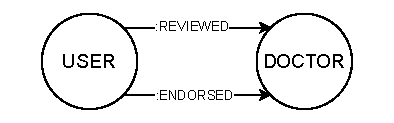
\includegraphics[scale=1.7]{./resources/neo4j.pdf}
    \caption{GraphDB structure for HealthHub}
    \label{fig:neo4j-structure}
\end{figure}

Our graph database (Figure~\ref{fig:neo4j-structure}) models two main entities:

\begin{itemize}
  \item \texttt{User}
  \item \texttt{Doctor}
\end{itemize}

Each node retains the MongoDB identifier to maintain consistency across databases. Neo4j is used selectively, focusing on relationship patterns and core attributes needed for traversal and inference, while full entity details remain in MongoDB.

The graph database plays a central role in modeling the social structure of the platform and is exploited in two main ways:
\begin{enumerate}
  \item As a \textbf{recommendation engine}, suggesting doctors to users based on graph proximity and shared review patterns.
  \item As a \textbf{search optimization layer}, improving query efficiency by leveraging graph traversal capabilities.
\end{enumerate}

Due to the lack of geographic data, we approximate location by leveraging graph proximity, under the assumption that users typically visit doctors near them. This enables us to infer locality-aware clusters and improve personalization without explicit spatial attributes.

\subsection{Node Types}

Neo4j stores only a minimal subset of each entity:
\begin{itemize}
  \item \textbf{User} nodes: \texttt{name}, \texttt{\_id}.
  \item \textbf{Doctor} nodes: \texttt{name}, \texttt{specializations}, \texttt{\_id}.
\end{itemize}

This lean representation minimizes redundancy while supporting all graph-based operations.

\subsection{Relationships}

We define two types of directed edges:
\begin{itemize}
  \item \textbf{:REVIEWED} — if user \texttt{U} has reviewed doctor \texttt{D}, then a \texttt{:REVIEWED} relationship is created from $U$ to $D$:  
  \[
    \texttt{U} \xrightarrow{\texttt{:REVIEWED}} \texttt{D}
  \]

  \item \textbf{:ENDORSED} — if user \texttt{U} endorsed doctor \texttt{D} (e.g., marked them as a favorite or recommended), we store this with a \texttt{:ENDORSED} relationship:  
  \[
    \texttt{U} \xrightarrow{\texttt{:ENDORSED}} \texttt{D}
  \]
\end{itemize}

These relations enable pattern discovery and inference. Spatial behavior is indirectly modeled through interaction patterns, which often reflect geographic closeness.

\section{Distributed Database Design}

\subsection{Replica Set Deployment}

\begin{figure}[t]
    \centering
    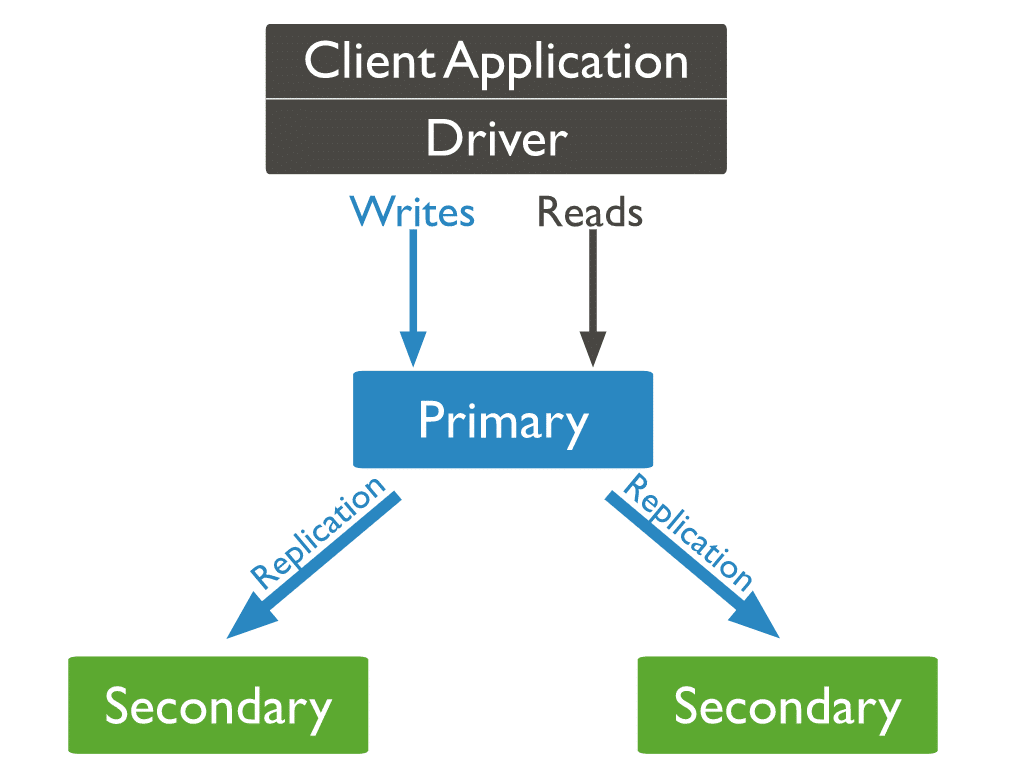
\includegraphics[scale=0.2]{./resources/mongo_replica.png}
    \caption{MongoDB Replica Set Structure}
    \label{fig:mongo-replica}
\end{figure}

We were given access to a cluster composed of three nodes. On each node, we deployed a MongoDB instance as part of a replica set. Neo4j was deployed in standalone mode, as replication requires the Enterprise edition, which was not available.

In the MongoDB replica set, only the \textbf{primary node} handles write operations. Each write is logged in the primary’s \emph{oplog} (operation log), which is then replicated to the \textbf{secondary nodes}. These secondaries apply the operations in the same order to maintain a consistent dataset. While all members of the replica set can serve read operations, by default, the application is configured to read from the primary node to preserve strong consistency.

\paragraph{Consistency Level}

Consistency across replicas is determined by the acknowledgment settings used during read and write operations. Our system adopts a hybrid consistency strategy:

\begin{itemize}
  \item The \texttt{write concern} is set to \texttt{w:1}, meaning that a write is acknowledged as soon as it has been applied by the primary node.
  \item The \texttt{read concern} is generally set to \texttt{local} (\texttt{r:1}), allowing reads from the local state of a node, which may not reflect the latest writes.
  \item However, for critical data such as a doctor's availability schedule, we explicitly enforce \texttt{readConcernLevel=majority} to ensure that only the most up-to-date and replicated information is retrieved.
\end{itemize}

This approach enables us to maintain \textbf{eventual consistency} where acceptable — improving performance and reducing latency — while enforcing \textbf{strong consistency} only in the specific cases that require it. It provides a good balance between responsiveness and data reliability, especially in a system that emphasizes availability and user experience.

\paragraph{CAP Theorem Considerations}

Our architecture emphasizes the \textbf{Availability (A)} and \textbf{Partition Tolerance (P)} aspects of the CAP theorem. The system is designed to:
\begin{itemize}
  \item Remain accessible and operational even during node failures or network partitions.
  \item Avoid sacrificing user responsiveness, ensuring that essential features—like searching doctors or leaving endorsements—remain available under most failure scenarios.
\end{itemize}

\subsection{Sharding (Design Perspective)}

Sharding has not been implemented in the current system but was considered as a viable strategy to scale the document database in case of high demand.

\paragraph{Horizontal Partitioning Strategy}

Sharding would be employed solely on the MongoDB side, as distributing a graph database like Neo4j across nodes introduces significant traversal overhead that defeats its performance benefits.

We proposed the following sharding design:

\begin{itemize}
  \item \textbf{Doctors Collection}:
    \begin{itemize}
      \item \textbf{Shard Key}: \texttt{address.province}
      \item \textbf{Sharding Mechanism}: hash-based
    \end{itemize}
    This approach would evenly distribute documents geographically, avoiding load concentration in specific provinces.

  \item \textbf{Appointments Collection}:
    \begin{itemize}
      \item \textbf{Shard Key}: \texttt{appointmentDateTime}
      \item \textbf{Sharding Mechanism}: range-based
    \end{itemize}
    Optimized for time-range queries, this configuration would support efficient access to recent or upcoming appointments.
\end{itemize}

These design options would ensure balanced workloads and scalable query processing if user and appointment volumes significantly increase in the future.

\subsection{Handling Inter-database Consistency}

Given that we use both a document-oriented database (MongoDB) and a graph database (Neo4j), some redundancy exists across the systems. Certain information—such as user endorsements—must be stored and updated in both databases.

To ensure consistency, we follow a two-phase update pattern:
\begin{itemize}
  \item A write operation is first performed on MongoDB.
  \item Only if the MongoDB operation is successful, the corresponding write on Neo4j is triggered.
  \item If the Neo4j update fails, a rollback is initiated to restore the system to a consistent state.
\end{itemize}

This logic is managed using Spring’s \texttt{@Transactional} annotation, ensuring atomicity across operations. Additionally, asynchronous execution is enabled via \texttt{@Async}, allowing long-running updates to Neo4j to execute in separate threads, enhancing system availability.

\begin{figure}[!ht]
    \centering
    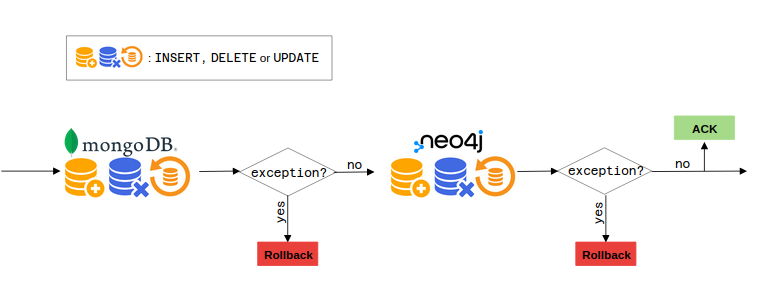
\includegraphics[scale=0.5]{./resources/rollback.png}
    \caption{Handling consistency between MongoDB and Neo4j}
    \label{fig:mongo-neo4j-sync}
\end{figure}

\paragraph{Eventual Consistency and Responsiveness}

The system is designed to tolerate brief inconsistencies between MongoDB and Neo4j. This decision improves performance and responsiveness—key aspects for a user-focused social system. Consistency is restored asynchronously and transparently, without impacting the user experience.
